\documentclass[spanish, fleqn]{scrartcl}
\usepackage[utf8]{inputenc}
\usepackage{babel}
\usepackage[paper=a4paper, top=2cm, left=2cm, right=2cm]{geometry}
\usepackage{tikz}
\usepackage{CIACcustom}
\usepackage{fourier}
\usepackage{amsmath, amsthm}
\usepackage{listings}
\usepackage{multicol}
\usepackage{fancyhdr}
\usepackage[urlcolor=blue, colorlinks]{hyperref}
\usepackage{booktabs,tabularx}
\usepackage{float}
\usepackage{ulem}

\newcolumntype{L}[1]{>{\hsize=#1\hsize\raggedright\arraybackslash}X}%
\newcolumntype{R}[1]{>{\hsize=#1\hsize\raggedleft\arraybackslash}X}%
\newcolumntype{C}[2]{>{\hsize=#1\hsize\columncolor{#2}\centering\arraybackslash}X}%

\pagestyle{fancy}
\fancyhf{}
\rhead{\pgfimage[width=2.5cm]{imagenes/logo-ciac.png}}
\chead{
  Apoyos Intensivos Guía N° 3\\
  IWI-131 Semestre I-2019 \\
  CIAC Casa Central
}
\lhead{\pgfimage[width=2.5cm]{imagenes/logo-usm.jpg}}
\rfoot{\LaTeXe / CIAC 2019}
\lfoot{Página \thepage}
\renewcommand{\headrulewidth}{0.5pt}
\renewcommand{\footrulewidth}{0.5pt}

\renewcommand{\ttdefault}{pcr}

%%% listings settings:
\definecolor{bggray}{rgb}{0.95,0.95,0.95}
\lstdefinestyle{consola}{
  backgroundcolor=\color{bggray},
  basicstyle=\small\ttfamily,
  frame=single,
  moredelim=[is][\bfseries]{[*}{*]},
  xrightmargin=5pt
}

\lstdefinestyle{mypy}{
  language=python,
  backgroundcolor=\color{bggray},
  basicstyle=\ttfamily\small\color{orange!70!black},
  frame=L,
  keywordstyle=\bfseries\color{green!40!black},
  commentstyle=\itshape\color{purple!40!black},
  identifierstyle=\color{blue},
  stringstyle=\color{red},
  numbers=left,
  showstringspaces=false,
  xrightmargin=5pt,
  xleftmargin=10pt
}

\newtheorem{CIACdef}{Definición}

\begin{document}
\vspace*{.3cm}

\section{Algoritmos útiles e interesantes (y divertidos también)}

Varios algoritmos recurrentes que se encuentran en este ramo se pueden programar de distintas formas y son útiles para la vida ingenieril y cotidiana.

\subsection{Cálculo de promedio}

Este algoritmo consta de dos contadores, \texttt{suma} y \texttt{cont}, que almacenan el numerador y denominador de la fórmula del promedio.

$$ \frac{\sum_{i=1}^{n} x_{i}}{n} $$

Donde $x_i$ es la cantidad ingresada de uno de los $n$ datos con que se calculará el promedio. En Python, un programa y su ejemplo sería


    \lstinputlisting[
    style  = mypy,
    caption= \texttt{promedio.py}]{Code/promedio.py}
    
Al correr el programa se tiene

\begin{lstlisting}[style=consola]
Ingrese dato: [*7*]
Ingrese dato (-1 para salir): [*5*]
Ingrese dato (-1 para salir): [*3*]
Ingrese dato (-1 para salir): [*12*]
Ingrese dato (-1 para salir): [*-1*]
El promedio de los datos es 6.8
\end{lstlisting}

\subsection{Encontrar un máximo o mínimo}

Consta de una variable \texttt{maximo} que guarda el dato numérico más alto que ingresa el usuario (o se lee de alguna estructura como verá más adelante en el ramo). Opcionalmente se puede guardar una variable que asocie el número más alto con un nombre. 

Tome un ejemplo de donaciones realizadas por importantes filántropos, cuyo código es

    \lstinputlisting[
    style  = mypy,
    caption= \texttt{maximizacion.py}]{Code/maximizacion.py}

\begin{lstlisting}[style=consola]
Ingrese nombre del donador: [*Pedro*]
Ingrese donacion: [*12000*]
Ingrese nombre del donador (enter para salir): [*Anghelo*]
Ingrese donacion: [*15000*]
Ingrese nombre del donador (enter para salir): [*Miguel*]
Ingrese donacion: [*25000*]
Ingrese nombre del donador (enter para salir): [*Sandro*]
Ingrese donacion: [*600*]
Ingrese nombre del donador (enter para salir): 
La donacion mas alta fue de 25000 realizada por Miguel
\end{lstlisting}

Note que para encontrar el mínimo de los datos basta con modificar la inicialización de la variable \texttt{maximo} por \texttt{minimo=float('inf')} en la línea 1, y \texttt{monto<minimo} en la línea 5.

\subsection{Lectura de strings}

Para acceder al valor de un elemento de una estructura se usa \texttt{estructura[indice]}. En este caso, la estructura pasa a ser un string, y el indice un valor numérico que va desde 0 (primer elemento) a \texttt{len(estructura)-1} (que es el último elemento). También se puede acceder a los elementos de forma inversa, como es el caso de \texttt{estructura[-indice]}, donde el último elemento tiene índice -1.

Un ejemplo de esto es contar las vocales de una palabra ingresada por el usuario. El código es 

 \lstinputlisting[
    style  = mypy,
    caption= \texttt{lectura.py}]{Code/lectura.py}

\begin{lstlisting}[style=consola]
Ingrese palabra: [*Programacion*]
La palabra Programacion tiene 5 vocales
\end{lstlisting}


\vspace*{-0.4cm}
\section*{Pregunta 1}

\begin{enumerate}
    \item A continuación se presenta el ruteo correspondiente:
\begin{center}
    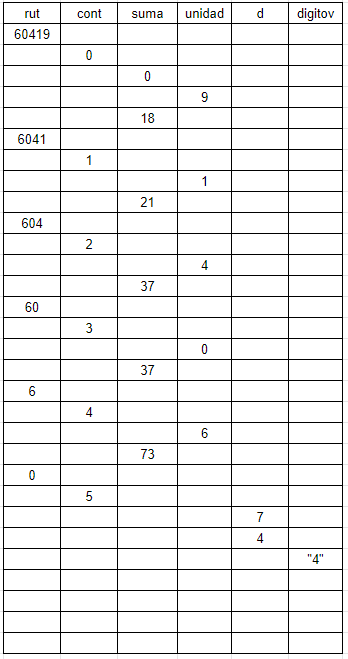
\includegraphics[scale=0.84]{Imagenes/ruteo_pauta}
\end{center}

    El programa imprime \texttt{4}.

    \item El código calculaba el dígito verificador del RUT. También era aceptable responder que, en base a cierto numero, este programa entrega un caracter que podría ser un dígito o una k.

\end{enumerate}

\newpage
\section*{Pregunta 2}

A continuación se presenta una forma posible de resolver el problema propuesto:
\lstinputlisting[
    style  = mypy,
    caption= \texttt{biblioteca.py}]{Code/p2.py}

\newpage
\section*{Pregunta 3}

A continuación se presenta una forma posible de resolver el problema propuesto:
\lstinputlisting[
    style  = mypy,
    caption= \texttt{tepyton.py}]{Code/p3.py}
\section{Matrices}

Las funciones solicitadas y el máximo correspondiente (70600674) se calculan con el siguiente código

\lstinputlisting[style=mypy,caption=\texttt{matrices.py}]{Code/matrices.py}


\end{document}